% -*- coding: utf-8 -*-
\section{ATH-kurve}
Average Threshold of Hearing (ATH) beskriver den mindste lydstyrke det
menneskelige øre kan opfatte i de forskellige frekvensområder. Et plot
af ATH for forskellige aldersgrupper vises i figur
\ref{fig.ath}. Vores tilnærmede funktion beregnes som
\begin{equation}
ath(f) = \left\{
\begin{array}{ll}
1                         & \textrm{, hvis } f \leq 20\\
-\log_{10}(f) 0.2775 + 1& \textrm{, hvis } 20 < f \leq 4000\\
0.0000625 freq - 0.25   & \textrm{, hvis } 4000 < f \leq 20000\\
1                         & \textrm{, hvis } f > 20000
\end{array} \right.
\end{equation}

og er vist i figur \ref{fig.vores-ath}.
\begin{figure}[h!]
\begin{center}
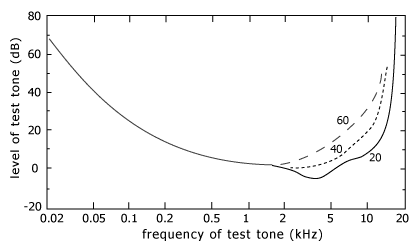
\includegraphics[width=12cm]{ATH}
\end{center}
\caption{Average Threshold of Hearing}
\label{fig.ath}
\end{figure}
\begin{figure}[h!]
\begin{center}
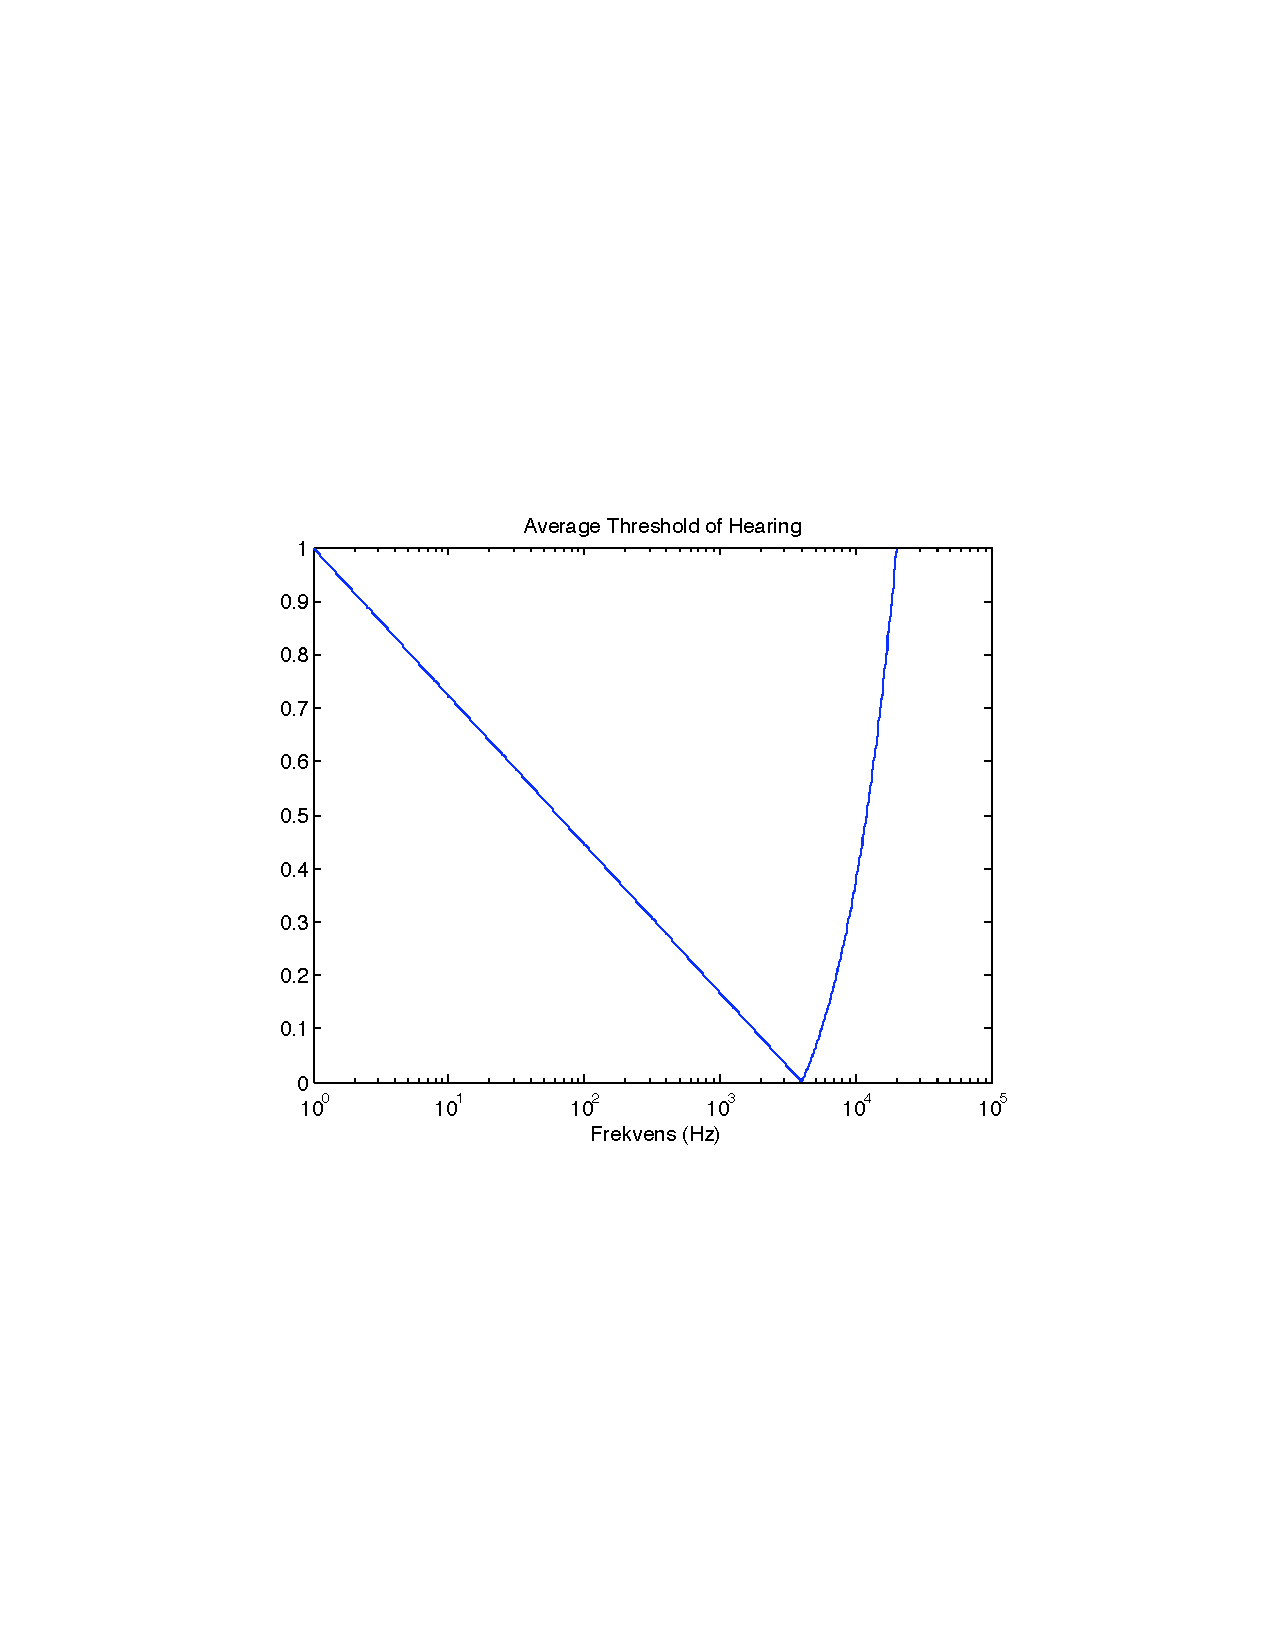
\includegraphics[width=12cm]{vores-ath}
\end{center}
\caption{Vores tilnærmede funktion til Average Threshold of Hearing}
\label{fig.vores-ath}
\end{figure}

